% \documentclass[12pt,draftclsnofoot,peerreview,onecolumn]{IEEEtran}
\documentclass[journal,comsoc,onecolumn, 12pt,draftclsnofoot]{IEEEtran}
\usepackage[T1]{fontenc}
% \usepackage{cite}
% \usepackage{amsfonts}
\usepackage{amssymb}
\usepackage{amsmath}
\interdisplaylinepenalty=2500
\usepackage{filecontents}
\usepackage{url}
\usepackage{bm}
\usepackage[square,sort,comma,numbers]{natbib}
\usepackage{subfigure} 
% \usepackage{caption}
% \usepackage{subcaption}
\usepackage[colorlinks,
  linkcolor=black,
  anchorcolor=blue,
  citecolor=black
  ]{hyperref}
\ifCLASSINFOpdf
 \usepackage[pdftex]{graphicx}
\else
 \usepackage[dvips]{graphicx}
\fi

% correct bad hyphenation here
\hyphenation{op-tical net-works semi-conduc-tor}

\renewcommand{\citedash}{--}

\DeclareMathOperator*{\argmax}{arg\,max}

\begin{document}
%
% paper title
% can use linebreaks \\ within to get better formatting as desired

\title{Entropy Minimization Based Symbol Timing
\\and Carrier Frequency Recovery}
% \author{\IEEEauthorblockN{Xiao Liu and Jean-Fran\c{c}ois Bousquet }
% \IEEEauthorblockA{Electrical and Computer Engineering\\
% Dalhousie University\\
% Halifax, B3H 4R2, Canada\\
% Email: x.liu@dal.ca}}
\author{Xiao~Liu,~\IEEEmembership{Student Member,~IEEE,}
%         John~Doe,~\IEEEmembership{Fellow,~OSA,}
        and~Jean-Fran\c{c}ois~Bousquet,~\IEEEmembership{Member,~IEEE}% <-this % stops a space

\thanks{Manuscript received November, 2017; revised xxxx xx, 2018. This project was supported by the Atlantic Innovation Fund \#Project \#203162.}
\thanks{The authors are with the Department of Electrical and Computer Engineering, Dalhousie University, Halifax,
NS, B3J 1Z1, Canada (e-mail: \{x.liu, jbousquet\}@dal.ca).}% <-this % stops a space
% \thanks{J. Bousquet is with Dalhousie University.}% <-this % stops a space
}

% The paper headers
% \markboth{IEEE Transactions on Communications,~Vol.~xx, No.~x, xxxxxx~2017}
{Shell \MakeLowercase{\textit{et al.}}: Entropy Minimization Based Symbol Timing and Carrier Frequency Recovery}

% make the title area
\maketitle


\begin{abstract}
This paper presents a new entropy minimization criterion for both symbol timing and carrier frequency recovery in  wireless receivers.
The synchronization is achieved by minimizing the entropy estimated from the eye diagram and the constellation diagram. 
A custom entropy estimation algorithm is proposed to achieve fast entropy estimation of the synchronization parameters.
A unified synchronization algorithm implementation with reduced complexity is proposed and its performance is evaluated in controlled conditions, as well as with realistic measurement data acquired during an underwater communication sea trial.
Compared to maximum likelihood based methods, it is shown that entropy minimization based algorithms have superior performance in various communication conditions, particularly when the channel is non-Gaussian or nonlinear.

% During the parameter search, when the perfect synchronization is achieved, the entropy will reach a sharp global minimum, indicating the least intersymbol interference or a restored constellation diagram. 
% The minimized entropy indicates a regular pattern with the least interference, that is where the signal is synchronized and recovered correctly.
% In the synchronization parameter search, the corresponding entropy reaches a sharp global minimum when the signal is recovered correctly.
% Unlike other synchronization methods, this unified criterion can be used to build an all-in-one synchronizer with high accuracy.
% The feasibility of this method is proven using a theoretical analysis and supported with numerical simulation. 
\end{abstract}

% {\bf Keywords:} 
\begin{IEEEkeywords}
Entropy minimization, symbol timing, carrier frequency recovery, synchronization.
\end{IEEEkeywords}

\IEEEpeerreviewmaketitle

\section{Introduction}
\label{sec:intro}
\IEEEPARstart{I}{n} coherent wireless communications systems, synchronization is a key operation at the receiver.
It is usually realized between the matched filter and the equalizer.
The two main functions of the synchronizer are symbol timing and carrier recovery.
The purpose of symbol timing recovery is to recover the symbol clock from the modulated waveform, so that it can down sample the waveform with the correct timing delay~(TD).
At the output of a matched filter sampled at the ideal instant, the signal will have maximum signal to noise ratio (SNR) and no intersymbol interference~(ISI)~\cite{mengali1997synchronization}.
Also, coherent demodulation of a passband signal requires the down converter to have exactly the same frequency as the carrier. 
In practice, the local oscillator frequency deviates from the input signal's carrier frequency.  
As such, this carrier frequency offset~(CFO) has to be compensated. 
In some applications, such as underwater acoustic communication, the channel may constantly change due to the time-variant channel or Doppler effect. 
Therefore a continuous estimation and compensation of the TD and CFO is essential to maintain the link reliability.

% \textbf{a summary of standard solutions }
Various synchronization algorithms have been proposed in the literature.
% They are generally characterized by their structures or the availability of training data.
They can be either feedforward or feedback depending on their configurations.
Also, the algorithms can also be categorized to data-aided (DA) or non-data-aided (NDA) according to the availability of training data.

% The \textit{feedforward} structure directly extracts the timing tone or CFO  from the incoming signal.
% Whereas the \textit{feedback} structure uses a timing (or frequency) error detector to derive an error signal and feeds it back to recover the synchronization parameters.
% On the other hand, 


% is supervised, otherwise it is unsupervised.
% This categorization is also known as \textit{data-aided} (DA), \textit{decision-directed} (DD) and \textit{non-data-aided} (NDA) 

Most synchronization algorithms follow the maximum likelihood (ML) criterion or its approximation.
For example, the O\&M algorithm \cite{Oerder1988}, a magnitude-squared nonlinear spectral line method exploiting the cyclostationary properties of the modulated signal, is one of the most commonly used NDA feedforward algorithm for symbol timing recovery.
It has been proven that this algorithm and its modifications can be asymptotically interpreted as ML estimators \cite{YanWang2002,Lopez-Salcedo2006}.
Also, the NDA Gardner timing error detector~\cite{Gardner1986} and its DA counterpart, the zero-crossing detector~\cite{gardner1988demodulator} can be derived from the ML criterion~\cite{Oerder1987}.
Regarding carrier recovery, the NDA feedforward frequency offset estimator proposed in~\cite{Wang2004} employs the fourth-order cyclostationary property, and still follows the ML criterion.
Various DA frequency offset algorithms attempt to maximize the inner product between the  training sequence and the data samples can be treated as ML estimators as well~\cite{mengali1997synchronization}.
The ML criterion assumes a Gaussian and leaner system, but it is not always satisfied in reality. 

% \textbf{What is scope of this paper }
% In this paper, we consider entropy minimizes (EM) as an alternative criterion for synchronization parameter estimation.
The primary contribution of this paper consists in the definition of a unified synchronization principle, the entropy minimization (EM). 
Specifically, the entropy of the eye diagram is evaluated for symbol timing recovery, and the entropy of the constellation is measured for carrier frequency recovery.
In both applications, the synchronization parameter that leads to a minimum entropy value is considered to be optimum.
% and the objective function based on this criterion is applied to both symbol timing and carrier frequency recovery.
% Like the ML criterion, it aims to optimize a unified objective function.
The algorithms that will be applied in this work are NDA and implemented in a feedforward structure, but they can be extended to other configurations under the same criterion.
Note that it has been shown in~\cite{Pedzisz2006} that the carrier frequency offset of the phase-shift keying (PSK) modulated signals can be recovered by minimizing the entropy of the instantaneous phase probability density function.
% Also, it has been reported that the error entropy minimization algorithms can be applied for channel equalization \cite{Santamaria2002}. 
However, to the authors' knowledge,  the unified criterion for both symbol timing and carrier recovery has not been proposed before. 

Since Shannon's work~\cite{Shannon1948}, entropy is an important concept in information theory. 
However, it is rarely used in practice, because it is difficult to estimate directly from samples without a model~\cite{Bercher2000,Santamaria2002}.
Exceptionally, in the study of physiological data, researchers use simplified approximate entropy (ApEn)~\cite{Pincus1991}, or sample entropy (SampEn)~\cite{Richman2000} to estimate the complexity of the time series.
As a second contribution of this work, we will propose a customized entropy estimation algorithm to accelerate the synchronization searching,
where the kernel function is used to estimate the normalized quadratic R\'enyi entropy~\cite{Santamaria2002,Huang2008}.
The third contribution of this work consists in demonstrating the performance in controlled conditions as well as in realistic underwater acoustic propagation conditions.  
The effect of various channel impairments will be analyzed on the system performance.  
% PMF not PDF
% Unlike these systems, this paper focuses on
%  \textbf{contributions}
% The contribution of this work is summarized as below.
% 1)~The entropy minimization (EM) criterion is studied for symbol timing and carrier frequency recovery.
% 2)~An ad-hoc entropy estimation algorithm is proposed for fast parameter estimation.
% 3)~The practical issues of EM based synchronization algorithms is discussed. 



This paper is organized as follows.
In Section \ref{sec:entropy},
an entropy minimization criterion for synchronization is introduced. 
In Section \ref{sec:cust_entp}, a customized fast entropy estimation algorithm is described. 
The algorithm implementation are presented in Section \ref{sec:imple}.
In Section \ref{sec:perfo}, the performance of the algorithms are evaluated in controlled conditions, and the algorithm is also applied to realistic data.  
Finally, conclusions are drawn in Section \ref{sec:conc}.
% \clearpage
%%%%%%%%%%%%%%%%%%%%%%%%%%%%%%%%%%%%%%%%%%%%%%%%%%

\section{Entropy Minimization Based Synchronization}
\label{sec:entropy}
In this section, the signal model that will be used through this paper is presented.
The standard ML criterion is briefly introduced in comparison to the EM criterion.
% we are going to use through this article.
Then, the application of the EM criterion to symbol timing and carrier frequency recovery using the eye diagram and constellation diagram will be explained.
% An ad-hoc entropy estimation algorithm is proposed in the last part of this section for fast synchronization parameter search.
\subsection{Signal model }  

% There are other forms of definitions or expressions of entropy that won't be detailed here.
% We will focus on how entropy can be applied in symbol timing and carrier frequency recovery.

In this work, it is assumed that the signal is transmitted using coherent modulation schemes, such as PSK, QAM (quadrature amplitude modulation) or CPM (continuous phase modulation), with an alphabet size of \(M\), where \(M\) is usually a power of 2.
The received binary information follows an independent identical distribution.
The modulated data is pulse shaped to limit the bandwidth occupancy.
The root-raised-cosine (RRC) filter is chosen as the pulse shaping filter at the transmitter, which is designed under the Nyquist criterion, 
such that there is no ISI at the proper sampling instants.

\begin{figure*}[ht]
\centering
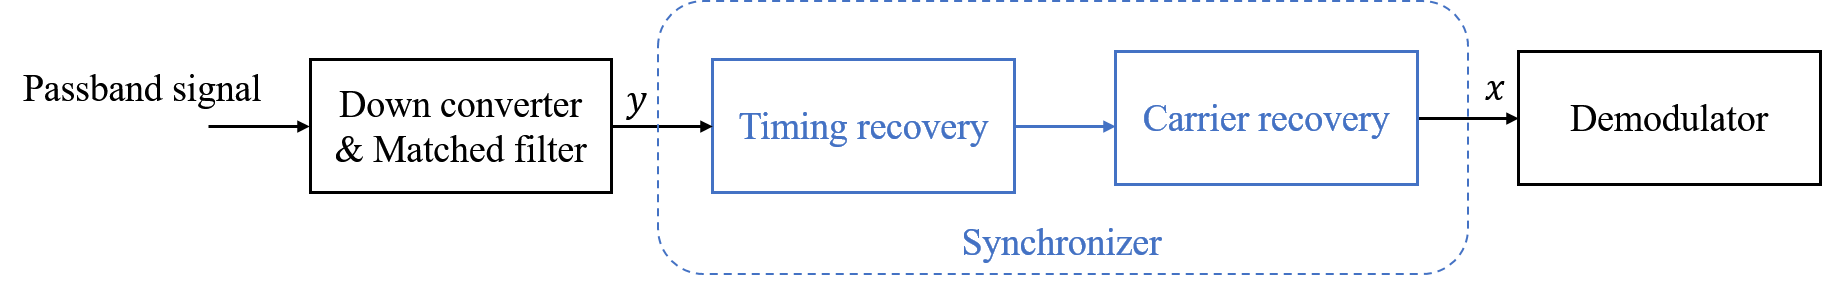
\includegraphics[width=5.5 in]{pic/sys_conf.png}
\caption{Block diagram of the receiver configuration.}
\label{fig:sysconf} 
\end{figure*}

Fig. \ref{fig:sysconf} shows the block diagram of the receiver configuration.
The down conversion is done first, and CFO may be present at its output.
The matched filter is the same RRC filter used in pulse shaping, so the overall filter becomes a raised-cosine~(RC) filter. 
Then, timing recovery is applied prior to carrier recovery.
Assuming that the timing is known, the decimated samples (usually one or two samples per symbol) are sufficient for CFO recovery.
Also, if the symbol timing is recovered first, the carrier recovery will have less computational burden due to the decimation of samples.
Therefore, the preferred sequence in this work is to apply symbol timing before carrier frequency recovery.

The $i$-th data samples \(x_i\) after timing and carrier frequency recovery can be expressed as
\begin{equation}
{x_i}( \tau ,{f_\Delta }) = y(iT +  \tau ){e^{ - j2\pi {f_\Delta }iT}},
\end{equation}
where \(y\) is the output of the matched filter, \(\tau\) and \(f_\Delta\) are the TD and the CFO respectively.


\subsection{Maximum Likelihood Versus Entropy Minimization}
Conventional synchronization methods intend to maximize the likelihood function.
For instance, in the NDA symbol timing recovery, this criterion yields an objective function~\cite{mengali1997synchronization}
\begin{equation}
\Lambda(\tau) =\sum\limits_{i = 1}^N {{{\left| {{x_i}( \tau )} \right|}^2}}, 
\end{equation}
while the DA carrier frequency recovery often uses an objective function~\cite{mengali1997synchronization} equal to
\begin{equation}
\Lambda ({f_\Delta })=\left| \sum\limits_{i = 1}^N {{{{c_i^*{x_i}(\tau ,{f_\Delta })}}}} \right|, 
\end{equation}
where \(c_i^*\) is the complex conjugate of the \(i\)-th training data.
These two objective functions are actually aimed at maximizing the energy of the data sample set.
This type of estimation method uses second-order statistics of the samples and is suitable for linear channels with Gaussian noise.
In a nonlinear propagation channel, where the AWGN condition is not respected, a criterion considering the higher order statistics would be more appropriate.
% Without the linearity and Gaussianity assumption, a criterion considering the higher order statistics would be appropriate.
The entropy is a measure of randomness or uncertainty of this signal, and it is a function of the signal probability density function (PDF).
As demonstrated in \cite{Santamaria2002}, by using entropy instead of likelihood function, the higher order statistics are taken into consideration.

The Shannon entropy is a measure of the quantity of information  embedded in a signal.
% In fact, we can also consider it as a measure of randomness or uncertainty of this signal.
% The most common approach to estimate the entropy is defined below.
% This Shannon entropy of discrete signal is defined below.
Assuming \(M\) possible observations of a one-dimensional discrete signal, with \(p_k\) representing the probability of the \(k\)-th possibility, the Shannon information entropy \(H_S\) is expressed as \cite{Shannon1948}
\begin{equation}
H_S =  - \sum\limits_{k = 1}^M {{p_k}\log {p_k}}.
\label{eq:entropy}
\end{equation}
The base of the logarithmic function is usually chosen to be 2, and the corresponding entropy unit is expressed in \textit{bits}.
% Next, we will use entropy as a metric to evaluate the eye diagram and constellation diagram.

\subsection{Eye Diagram Entropy and Symbol Timing Recovery}
\label{sec:eye_entp}
To recover the symbol timing, the entropy of the eye diagram is utilized. 
% The eye diagram is a graphical illustration that consists of many periodically overlaid traces of short windows of a signal.
% Normally, the length of the segment is one or two symbol periods. 
% The symbol timing recovery problem can be then interpreted as finding the adequate timing instant on the eye diagram.
Ideally, the down-sampling instant should be located in the middle of the eye diagram where the eye opening reaches its maximum.
The symbol timing recovery problem can be then interpreted as adjusting the timing instant with a proper delay (TD) on the eye diagram.
% Fig. \ref{fig:eyediagram} is an eye diagram for a BPSK signal overlaid at each symbol period.
% The binary data is shaped using raised-cosine pulses with a roll-off factor of 0.5.

We define the \textit{eye diagram entropy} as the entropy at a certain timing instant on the eye diagram.
Assuming no noise and perfect symbol timing (no ISI),
% The ISI can be eliminated if sampling in the middle of the eye diagram.
the samples can only be distributed within \(M\) possible symbols equally.
The probability that the samples belong to the $k$-th symbol is \(p_k=1/M\).
Substituting the probability into~(\ref{eq:entropy}), we have the minimum eye diagram entropy
\begin{equation}
\min{H_{eye}} =  - \sum\limits_{k = 1}^M {{\frac{1}{M}}\log_2 {\frac{1}{M}}}=\log_2 {M},
\label{eq:entropy_mid}
\end{equation}
which is exactly the same as the amount of information carried by each symbol.
% If the pulse shaped symbols are sampled at the ideal sampling instants, 
% there is no ISI and the entropy is minimized.
% With Nyquist pulse shaping, there is no ISI in the middle of the eye diagram, so the ISI is not considered in~(\ref{eq:entropy_mid}).
If the signal sample is deviating from the correct timing instant, adjacent pulses will be mixed into the samples.
Since each pulse from adjacent symbols carries the same amount of information, the maximum entropy of a given timing instant can be
\begin{equation}
\max{H_{eye}} =  N_{span}\log_2 {M},
\label{eq:entropy_neb}
\end{equation}
where \(N_{span}\) is the span of the RC filter in symbols.
It is \(N_{span}\) times higher than the entropy measured in the middle of the eye diagram.

There may be existence of local minimum which will be addressed later in this paper,
but one can conclude that the entropy of an eye diagram comes to a global minimum in the middle of the eye.
Therefore, the symbol timing recovery can be approached by searching the timing instant with the minimum eye diagram entropy.


\subsection{Constellation Diagram Entropy and Carrier frequency Recovery}
\label{sec:const_entp}
When the passband signal is converted to baseband, the complex data can be visualized as a constellation diagram.
However, if the frequency of the local oscillator is  different (even very small) from the carrier of the signal, the resulting constellation diagram is rotating and cannot be demodulated.
We will focus on recovering a CFO that is smaller than the symbol rate, since for extremely large CFO, a preceding coarse carrier recovery is usually required.

If the down converted signal is impaired by CFO, it exhibits increased randomness in the constellation diagram, which can be measured by the \textit{constellation diagram entropy}.
% The increased randomness in the constellation diagram is due to the CFO and the resulting rotating constellation. 
% is unlike the eye diagram, where ISI.
% This randomness can be measured by the \textit{constellation diagram entropy}.
% Assuming perfect timing recovery, the constellation diagram entropy reaches to a minimum when there is no CFO.
% So, the expression of its minimum value is the same as~(\ref{eq:entropy_neb}).
The entropy has a global minimum corresponding to a zero CFO, and its value is equal to the amount of the information carried by the symbol, which is the same as~(\ref{eq:entropy_neb}).
The entropy upper limit can be achieved when the CFO or the number of samples is large enough,
such that the accumulated signal phase error is greater than the minimum phase difference of the signal modulation scheme. 
More discussion on entropy based carrier recovery can be found in \cite{Pedzisz2006}.
% add content from my wuwnet paper
% The probability density function (PDF) of its instantaneous phase can be used to estimate the entropy, and with the help of
It is important to note that, like the symbol timing recovery, the carrier frequency recovery can be achieved by searching the frequency with minimum constellation diagram entropy.
In the next two sections, a methodology to implement this unified criterion will be described.

\section{Customized Fast Entropy Estimation Algorithm}
\label{sec:cust_entp}
Entropy based algorithms are rarely used in signal processing because of their complexity~\cite{Bercher2000}.
% To develop practical entropy minimization based synchronization algorithms, a fast entropy estimation method is required.
% from the definition: histogram based estimation
According to the Shannon entropy equation~(\ref{eq:entropy}), the entropy is a function of the sample PDF, and one common technique is to use the histogram for PDF estimation.
The histogram is a simple visualization of data distribution where bins are defined, and the number of data points within each bin is tallied. 
However, the estimation of the PDF and the summation of multiple logarithm operations have high computational complexity.
In this section, we propose a fast customized entropy estimation algorithm that is suitable for EM based synchronization parameter recovery. 

To solve this problem, some researchers turned to alternative definitions of entropy, particularly, the R\'enyi entropy.
The R\'enyi entropy  with parameter \(\alpha\) is defined as \cite{renyi1961measures}
\begin{equation}
H_{R }={\frac {1}{1-\alpha }}\log {\Bigg (}\sum _{k=1}^{M}p_{k}^{\alpha }{\Bigg )}.
\label{eq:renyi}
\end{equation}
As explained in \cite{Bromiley2004}, when $\alpha~\to~1$, the R\'enyi entropy tends to Shannon entropy.
Following common practice for example used in \cite{Santamaria2002}, the quadratic R\'enyi entropy ($\alpha=2$) is chosen in this work for its simplicity.
In this case, (\ref{eq:renyi}) reduces to
\begin{equation}
H_{R2 }=-\log {\Bigg (}\sum _{i=1}^{M}p_{k}^{2 }{\Bigg )}.
\label{eq:renyi2}
\end{equation}
Note that in (\ref{eq:renyi2}), the logarithmic function is  external to the sum of the quadratic probabilities.
Because the logarithmic function is monotonic, minimizing (\ref{eq:renyi2}) is equivalent to maximizing its internal portion.
% \textit{information potential} $V$
% \begin{equation}
% V=\sum _{i=1}^{k}p_{i}^{2 }.
% \end{equation}

The \textit{kernel density estimation} is used to estimate the probabilities.
Given a set of \(N\) samples, \(i=1, \dots, N\), the sample PDF at an observation \(\xi\) can be estimated by~\cite{Principe2000a}
\begin{equation}
{ p(\xi)={\frac {1}{N}}\sum _{i=1}^{N}K_{r}\left(\xi-x_i\right)},
\label{eq:kernel}
\end{equation}
where $K_r(\cdot)$ is a kernel function with a positive parameter $r$.
Then, substitute (\ref{eq:kernel}) into (\ref{eq:renyi2}) and after some simplification, we have
\begin{equation}
H_{R2 }=-\log {\Bigg (}\frac{1}{N^2}\sum _{i=1}^{N}\sum _{j=1}^{N}K_{r}\left(x_i-x_j\right){\Bigg )}.
\end{equation}
Among various kernel functions, the simplest top-hat kernel is used to accelerate the computation.
This kernel function is given by
\begin{equation}
{\displaystyle K_{r}(x)={\begin{cases}1,&|x|\leq r\\0,&{\mbox{otherwise.}}\end{cases}}}
\end{equation}
% Despite its computational complexity, a major problem with histograms is that the choice of binning can have a side effect on the results.
% This interesting feature inspired us to develop a new ad-hoc entropy estimation algorithm for our application.

Now, the entropy can be estimated by  measuring the distances between samples instead of using the histogram.
% The proposed algorithm measure the aggregation degree of data samples by measuring the Euclidean distances between samples.
% The number of data samples $x_i$ under observation is denoted as \(N\), 
The proposed entropy estimation algorithm is summarized as:
\begin{enumerate}
\item Calculate all the distances \(d_{ij}\) between each sample pair \(x_i\) and \(x_j\), where \(1\le i<N\) and \( i<j \le N\). We have
 \begin{equation}
d_{ij}=\left\|x_i-x_j \right\|,
\label{eq:distance}
\end{equation}
where \(\left\| \cdot \right\|\) represents the Euclidean norm.
\item Define a threshold \(r_{ag}\) \((r_{ag}>0)\) and count the number of \(d_{ij}\) that satisfy $d_{ij}>r_{ag}$, and denote the count as $H_{sp}$.
\item After normalization, the modified R\'enyi entropy (MRE) is given by
\begin{equation}
H_{MRE}= \frac{ H_{sp}}{ N(N-1)/2}.
\label{eq:entorpy_ad}
\end{equation}
\end{enumerate}


The entropy \(H_{sp}\) can be alternatively interpreted as a measure of the sample aggregation,
and the threshold \(r_{ag}\) is used to determine if the two samples are closely located or separated.
Samples that aggregate into only a few groups indicate low entropy, whereas samples sparsely distributed suggest high entropy.
The choice of \(r_{ag}\) will be discussed later in this section.
% The last step normalizes $H_{sp}$, so that the modified R\'enyi entropy $H_{MR}$ does not depend on the number of samples.
The final result \(H_{MRE}\) is the modified version of the quadratic R\'enyi entropy  by dropping off the logarithmic function and using the kernel function for PDF estimation.
% We will call it the \textit{modified R\'enyi entropy} in the rest of the paper.
Because of the normalization, the value of $H_{MRE}$ is limited from 0 to 1 and is unitless.
This algorithm does not need to produce a histogram and does not need to compute the logarithm, making it much faster than the conventional entropy estimation method.

% Another interpolation 
% In the study of physiological time series data, researchers use  approximate entropy (ApEn) \cite{Pincus1991}, or sample entropy (SampEn) \cite{Richman2000}. to estimate the complexity of the time series.
% Instead of estimating the probability of samples, theses algorithms are looking for the probability of new patterns.
% In practice, the entropy increases for newer patterns. 

An example of the modified R\'enyi entropy estimation as a function of SNR is shown in Fig. \ref{fig:MRE}, where the histogram based Shannon entropy results are also plotted as a reference.
The samples consists of 1000 QPSK modulated (\(M=4\)) random symbols with unit power.

\begin{figure}[ht]
\centering
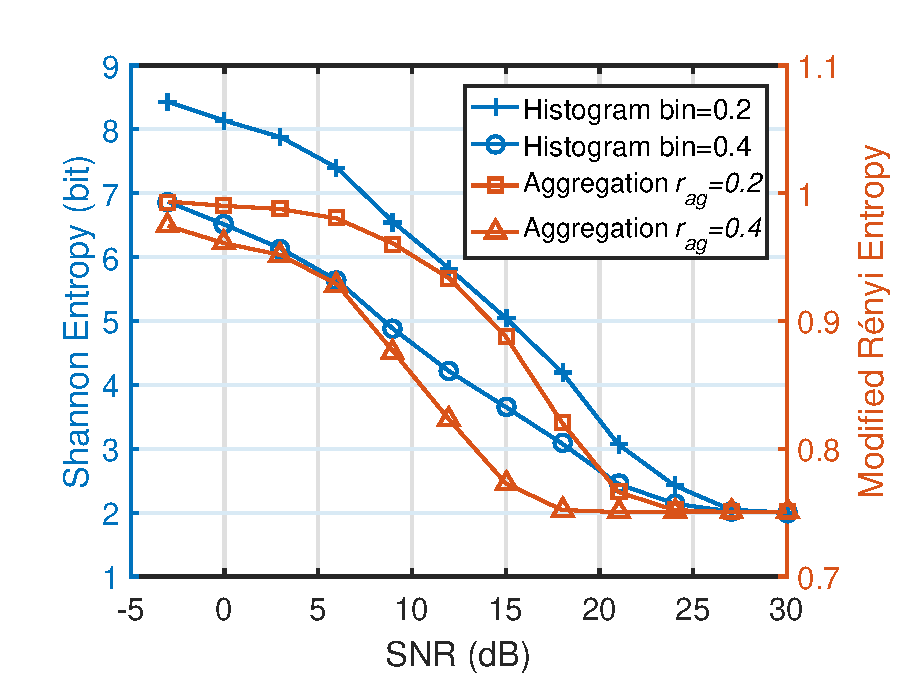
\includegraphics[width=3 in]{pic/H_MR.eps}
\caption{Entropy estimation using two algorithms.}
\label{fig:MRE} 
\end{figure}
% The additive white Gaussian noise (AWGN) is introduced, where the SNR sweeps from -3 dB to 30 dB.

In Fig. \ref{fig:MRE}, the 2D histogram based estimation is evaluated for a bin width of 0.2 and 0.4, and the same values are used for the aggregation threshold \(r_{ag}\) in the modified R\'enyi entropy estimation.
When the SNR is sufficiently high, the histogram based algorithm reaches the minimum. 
Its value is 2 bits in Fig. \ref{fig:MRE}, as was predicted by~(\ref{eq:entropy_mid}).

Next let's derive the minimum value of the modified R\'enyi entropy and compare it with the numerical results shown in Fig.~\ref{fig:MRE}.
Since the symbols are random, there are four groups of symbol points distributed in the constellation diagram, and each group has \(N/4\) samples.
The condition of $d_{ij}>r_{ag}$ can only be satisfied between samples with different constellation positions.
For two constellation positions, we have $H_{sp} = (N/4)^2$, so the total $H_{sp}$ will be $6 (N/4)^2$ if four constellation positions are considered.
Thus, the minimum value of the modified R\'enyi entropy is approximated by
\begin{equation}
H_{MR} \approx \frac{ 6 \left(N/4\right)^2}{N^2/2}=0.75.
\label{eq:adEntQPSK}
\end{equation}
which agrees with the results shown in Fig. \ref{fig:MRE}.


It can be seen that both algorithms are monotonic functions of SNR.
The decreasing entropy reflects the fact that the uncertainty of the system is reduced with the increasing SNR.
This property shows that the proposed algorithm can be used to measure the data randomness.

The choice of the threshold \(r_{ag}\) depends mainly on the noise level.
In Fig. \ref{fig:MRE}, the curve with \(r_{ag}=0.2\) reflects the change of randomness at high SNR, but saturates for low SNR region, in which case \(r_{ag}=0.4\) is preferred.
This is because the small threshold cannot differentiate the aggregation degree of large scale distributed data samples.
In practice, $r_{ag}$ can be set equal to the root-mean-square value of the noise.

% Similar with ApEn and SampEn algorithms, 
It is best to apply the modified R\'enyi entropy estimation using a few hundred samples,
because the required distance calculation exhibits quadratic growth with number of data samples. 
The computational pressure can be relieved by either skipping the distance calculation of aggregated samples or using other distance metric (Chebychev et al. \cite{Cha2007}).
However, this is not an issue in our application since a reliable synchronization  recovery with less data samples is always preferred, and it is an advantage in tracking the dynamic channel conditions. 
% 跟 histogram 比较性能
% r 选择有什么影响
%%%%%%%%%%%%%%%%%%%%%%%%%%%%%%%%%%%%%%%%%%%%%%%%%%
\section{Implementation of Symbol Timing and Carrier Frequency Recovery}
\label{sec:imple}
In this section, the entropy minimization criterion will be implemented to symbol timing and carrier frequency recovery.
Several practical issues are addressed and the
synchronization algorithms are discussed in detail. 
% The algorithms discussed here work in batch mode, which means the samples are processed block by block. 
% It is a direct result of the way entropy is estimated, however, after the initial acquisition, it is not difficult to adapt the algorithms to online mode with a sliding window.
% EM based symbol timing and carrier frequency recovery algorithms
% - configuration: batch search algorithms, timing first and then carrier recovery

\subsection{Symbol Timing Recovery} 
\label{sec:timing}
Symbol timing recovery can be implemented by searching the instant with minimum entropy in the eye diagram.
However, there are several practical issues that need to be addressed.
In the following discussion, we will focus on key issues: 
1)~addressing local minima in the entropy curve,  
2)~examining the timing recovery in presence of CFO, and 
3)~providing accurate timing recovery with low oversampling rate.

The entropy reaches a global minimum in the centre of the eye diagram, but in practice, when the timing instant is close to the symbol transition area, the entropy may go down and create local minima. 
The local minima will deteriorate the performance at low SNR conditions or when using gradient based search algorithms.
Since the entropy local minima occur when the sample magnitude is small, an additional minimum threshold can be introduced to eliminate data samples with small magnitudes in the entropy estimation.
With this idea, the algorithm in Section~\ref{sec:cust_entp} is amended:

\begin{enumerate}
\item Define a threshold \(r_{mg}\) \((r_{mg}>0)\) and build a new samples set where all samples with its magnitude greater than \(r_{mg}\) are included.
The number of samples in the new set is denoted as \(N_{mg}\).
\item Find out all the Euclidean distances \(d_{ij}\) between each sample pair \(x_i\) and \(x_j\) in the new sample set, where \(1\le i<N_{mg}\) and \( i<j \le N_{mg}\). 
\item Define a threshold \(r_{ag}\) \((r_{ag}>0)\) and count the number of \(d_{ij}\) such that $d_{ij}<r_{ag}$, and denote it as $H_{ag}$.
\item The bounded modified R\'enyi entropy (BMRE) is given by
\begin{equation}
H_{BMRE}= 1- \frac{ H_{ag}}{ N(N-1)/2}.
\label{eq:entorpy_ad2}
\end{equation}
\end{enumerate}



A typical case is given here to show how the entropy minimization based symbol timing recovery works.
The received frame consists of 400 QPSK modulated random symbols, 
which are pulse shaped by a RRC filter with a rolloff factor of 0.5 to generate a baseband complex envelop.
An AWGN channel is assumed with $E_s/N_0 = 18~\text{dB}$. 
After the matched filter, the eye diagram of the real component of the signal is plotted in the upper part of Fig. \ref{fig:timing}, and the entropy results estimated by both original and modified algorithms are shown in the lower part,
% as well as its entropy are plotted in , where
where the threshold $r_{ag}=0.25$ and \(r_{mg}=0.3\).
% The ad-hoc entropy estimation algorithm discussed in Section \ref{sec:adhoc} is used to evaluate the timing phase entropy of the eye diagram, where the threshold $r=0.25$.
% The timing phase entropy as a function of normalized timing offset is plotted as a solid red line in the lower part of Fig. \ref{fig:timing}, such that the two figures can be viewed under the same x-axis.

\begin{figure}[htbp]
\centering
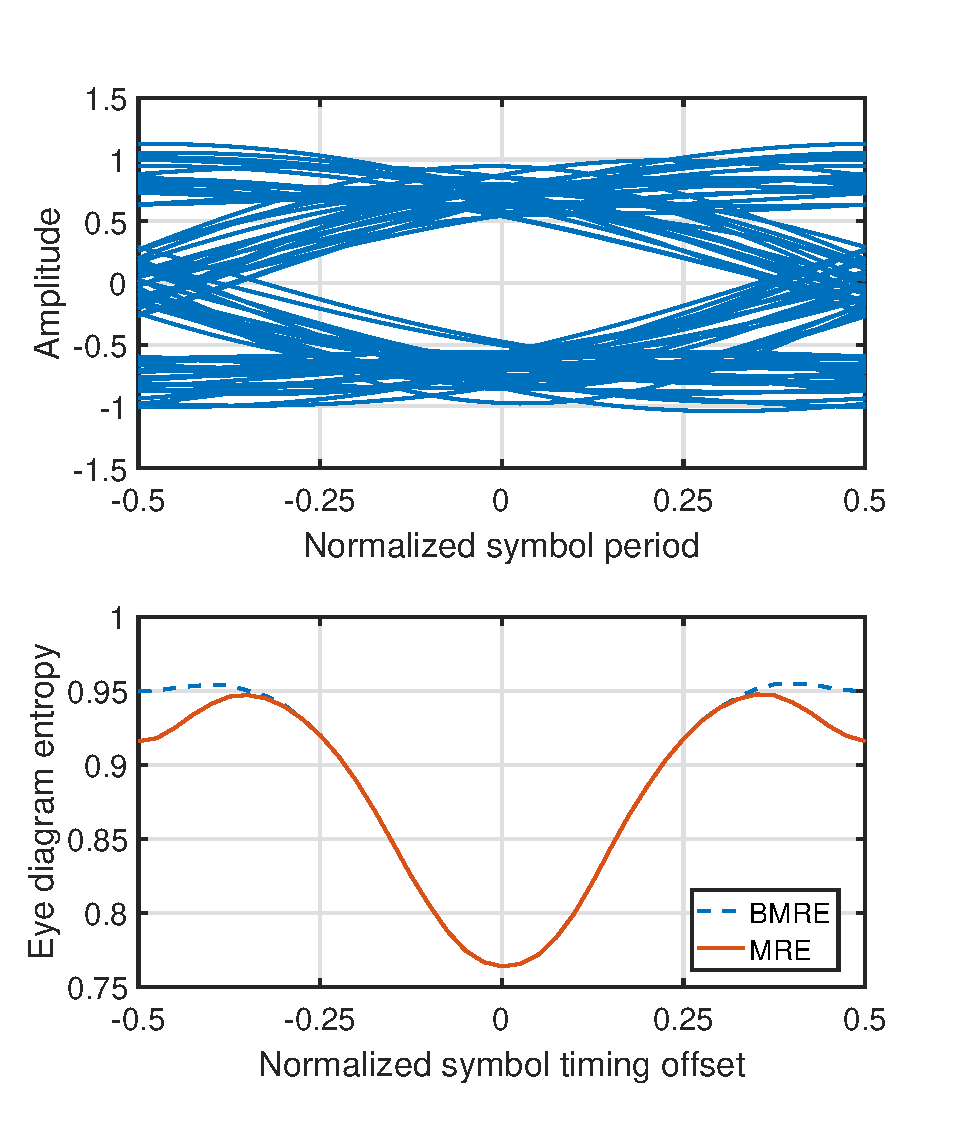
\includegraphics[width=3 in]{pic/timing.eps}
\caption{An typical eye diagram (upper) and the corresponding eye diagram entropy (lower).}
\label{fig:timing} 
\end{figure}

% \subsubsection{Entropy Local Minimum Removal}
From Fig.~\ref{fig:timing}, the entropy reaches a global minimum in the centre of the eye diagram, and its value is close to 0.75 as predicted by~(\ref{eq:adEntQPSK}).
With an increase of timing offset, the entropy increases, indicating  more randomness introduced by ISI.
When the timing offset is beyond $\pm 0.35$, the  entropy from the original algorithm goes down and creates a local minimum in the symbol transition area. 
% This is because the randomness reduces when the timing phase is close to the symbol transition area.
This phenomenon is also illustrated in the eye diagram, where the samples aggregate into three visible groups (with the amplitudes of \(\pm 1\) and 0).
% The local minimum is not a big issue if the SNR is high and a global search is applied, but it will deteriorate the performance in low SNR cases or when using gradient based search algorithms.

% The ad-hoc entropy estimated by the modified algorithm is also plotted in the lower part of Fig. \ref{fig:timing} where the \(r_{ag}=0.25\).
The entropy estimated by the amended algorithm coincides with the entropy of the original algorithm in most of the timing offsets, but the local minimum near 0.5 becomes flat.
As such, with the amended algorithm, the local entropy minimum due to the symbol transitions is removed and the symbol timing recovery can be achieve with higher accuracy.

% \subsubsection{Timing Recovery with Carrier Frequency Offset}
% In Fig.~\ref{fig:sysconf}, the timing recovery block is placed before carrier recovery, so the input signal of timing recovery may contain uncompensated CFO.
% We shall evaluate the viability of the proposed algorithm in such conditions. 
Next, the impact of timing recovery in presence of uncompensated CFO will be evaluated.  
Theoretically, the previous analysis of timing phase entropy still holds, but the CFO does introduce extra entropy in the estimation.
To understand how the CFO affects the eye diagram entropy, another simulation is conducted with the same parameters as in the early part of this section,
and the only difference is that a CFO at 1\% of symbol rate is introduced.
The eye diagram and the corresponding entropy are depicted in Fig. \ref{fig:timing_freq}.
      
\begin{figure}[ht]
\centering
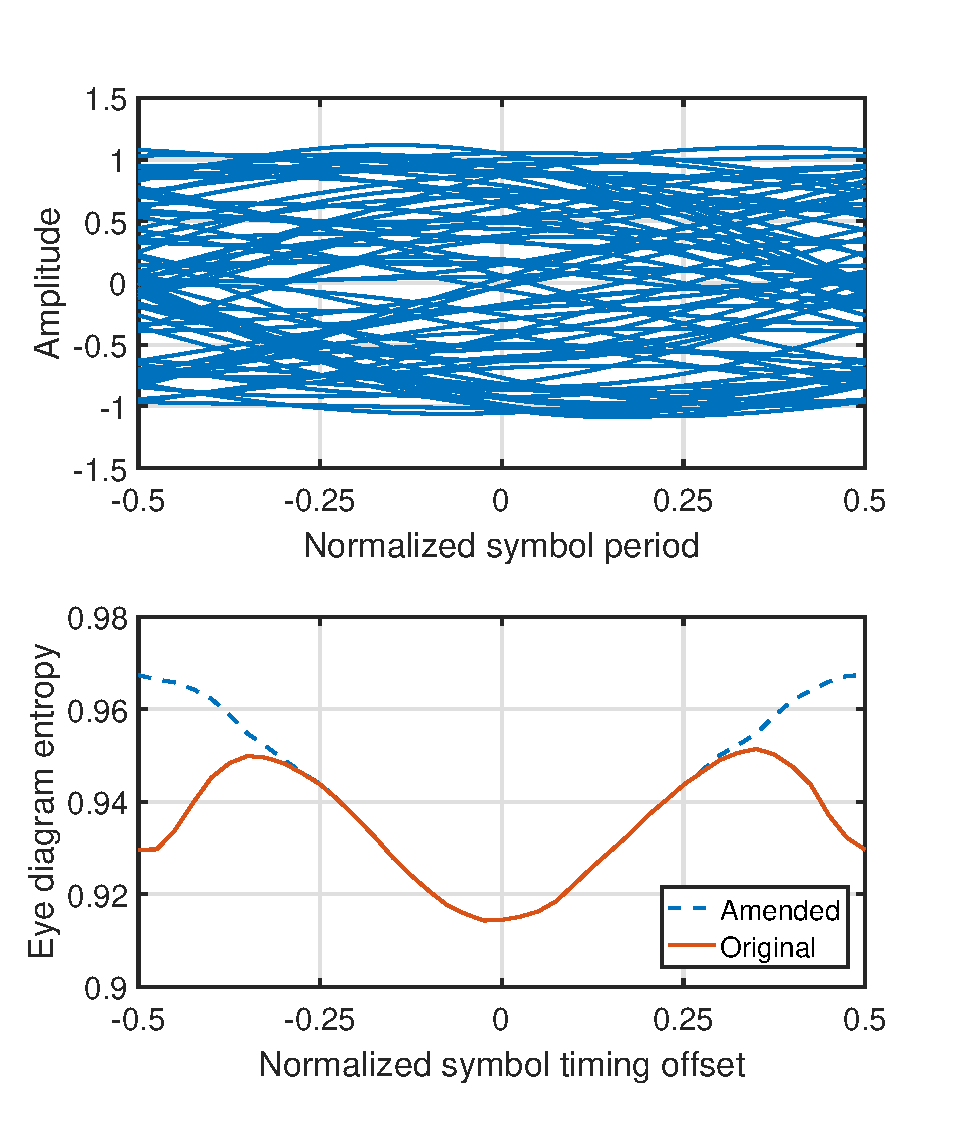
\includegraphics[width=3 in]{pic/timing_freq.eps}
\caption{An eye diagram with carrier frequency offset (upper) and the corresponding eye diagram entropy (lower).}
\label{fig:timing_freq} 
\end{figure}

The eye diagram in the upper part is messy and the eye is completely closed. 
There is no way to identify the centre of the eye or optimum timing instant by only looking at the eye diagram.
However, the entropy plot tells a different story.
Both the original and the amended algorithms have the same global minimum at 0 timing offset, which means the eye diagram entropy based algorithm is immune to the CFO,
but with the price that the entropy dynamic range is smaller than that without CFO.

The entropy plot at symbol transition area is also interesting.
With the original algorithm, the local minimum is more noticeable and may lead to a false timing offset estimate.
However, the amended algorithm shows superior performance:
the curve is not flat anymore but continue growing with the same gradient as a function of timing offset.
This feature shows a good adaptation of the modified algorithm, and proves that the `symbol timing before carrier recovery' configuration is feasible.

% \subsubsection{A Feedforward Timing Phase Estimator}
% \label{sec:timing_ff}
Next, a algorithm that can estimate TD for signal with low oversampling rate is proposed.
A global search for timing phase with minimum eye diagram entropy is not a elegant solution, especially when a high oversampling rate is not available.
Recall that the widely used feedforward symbol timing method, the O\&M algorithm, uses as low as 4 samples per symbol, and its TD is given by
\begin{equation}
\tau=\frac{T}{2\pi}\arg \left\{ {\sum\limits_{i = 1}^{N} {x_i^2{e^{ - j2\pi (i-1)/N_{sps}}}} } \right\},
\label{eq:om}
\end{equation}
where \(T\) is the symbol period and \(N_{sps}\) is the number of samples per symbol.
The operation \(\arg( \cdot )\) returns the phase angles, in radians.
The idea behind the O\&M algorithm is to apply discrete Fourier transform (DFT) to the squared signal \(x_i^2\),
and the TD is extracted from the angle of the resulting spectrum line at the symbol rate.

The same approach can be applied to EM based symbol timing algorithm.
To be specific, we can replace the squared signal term in O\&M algorithm with the eye diagram entropy,
such that the the TD can be found with
\begin{equation}
\tau  = \frac{T}{{2\pi }}\arg \left\{ {\sum\limits_{k = 1}^{N_{sps}-1} {H(k){e^{ - j2\pi (k-1)/N_{sps}}}} } \right\},
\label{eq:ff_alg}
\end{equation}
where \(H(k)\) is the eye diagram entropy at timing instant \(k\).
Note that (\ref{eq:ff_alg}) assumes that the entropy curve is symmetric to the centre of the eyediagram,
but it may not be maintained at  low SNR or multipath channel condition.
Its performance will be further discussed in Section \ref{sec:perfo}.

\subsection{Carrier Frequency Recovery}
This section will focus on the EM based carrier frequency recovery algorithm.
Like the symbol timing recovery discussed above, the proposed algorithm is NDA too.
The constellation diagram entropy is measured with the trial CFO in a certain range, and a global search is applied to find the global minimum. 
% The general idea is to multiply the signal by a local carrier with a trial CFO and calculate the corresponding constellation entropy.
% Then, sweep the trial CFO in a certain range and find the frequency with the minimum entropy value.
We will show the characteristics of the entropy curve first and then introduce a method that can cope with a problem due to sharp trough.

In Section \ref{sec:const_entp}, we found that the constellation entropy is almost constant when the CFO is greater than a frequency limit.
Within this frequency limit, the curve has a V-shape ``trough'' (negative peak) and the entropy global minimum is located in the middle of the trough.
For a given modulation scheme, the width of the trough is decided by the CFO $f_\Delta$, the symbol rate $1/T$ and the number of data samples $N$ in the window.
For example, the \(M\)-PSK modulated signal has a minimum constellation phase difference \(2\pi/M\).
The accumulated phase shift due to CFO is given by \(2\pi f_\Delta N T\).
The constellation entropy increases with the CFO until the accumulated phase shift is greater than the minimum constellation phase difference. 
Therefore, the trough range is given by
\begin{equation}
\left| {f_\Delta } \right| < \frac{1}{{MNT}}.
\label{eq:freq_limit}
\end{equation}
With CFO beyond this range, the entropy curve is going to be flat.


In (\ref{eq:freq_limit}), if \(N\) is equal to a few hundred, a given CFO that can fall into the entropy trough has to be on the order of 0.1\% of the symbol rate, which is relatively small compared to the CFO range that needs to be covered.
The resulting entropy curve as a function of trial CFO is basically flat with a sharp trough.
As a result, the linear search requires a very small step to achieve high frequency resolution, and the potential gradient descent algorithm cannot converge due to lack of gradient.
In other words, an efficient search algorithm cannot be applied. 

In order to cover a large estimation range without intensive computation, an algorithm that can expand the width of the trough is required.
% One possible way that can obtain a wide entropy trough
To increase the trough width, a possible solution is to use less data samples (reduce \(N\)), but that will lead to inaccurate PDF and entropy estimation.
Instead, a block average algorithm that is similar to~\cite{YuanlingHuang2007} is adopted to smooth the entropy curve:
\begin{enumerate}
\item Segment the \(N\) data samples into small blocks equally, where each of these block consists of \(L\) samples. 
% There can be overlaps for the blocks to improve the accuracy.
\item Estimate the entropy curve for each block.
\item Average the entropy results from all the blocks.
\end{enumerate}
If the CFO is constant through all the data samples, each block should possess the same entropy curve but with random fluctuation due to PDF estimation with insufficient samples.
By averaging the entropy curve using small blocks, a wide and smooth entropy trough is achieved.
The new trough is $N/L$ times wider than the original one.

With the same settings as in section \ref{sec:timing}, the numerical simulation of the constellation entropy with 400 samples, 50 samples and the entropy with block average are plotted as a function of the CFO in Fig. \ref{fig:freq_entp}.
Perfect symbol timing is assumed, and the CFO is swept within 1\% of the symbol rate.

% The frequency offset under recovery should be smaller than the symbol rate \cite{mengali1997synchronization}.
% To be specific, for \(M\)-PSK modulation schemes, if there are \(N\) samples with sampling interval of \(T_s\), the upper boundary of the frequency offset \(\Delta \omega_c\) is given by
% \begin{equation}
% \Delta \omega_c <\frac{2 \pi}{M N T_s}  
% \label{eq:f_lim}
% \end{equation}
% Regarding the case of QAM signals, the \(2 \pi/M\) in (\ref{eq:f_lim}) should be replaced by the minimum phase difference between their constellation points.

% \subsubsection{}

\begin{figure}[ht]
\centering
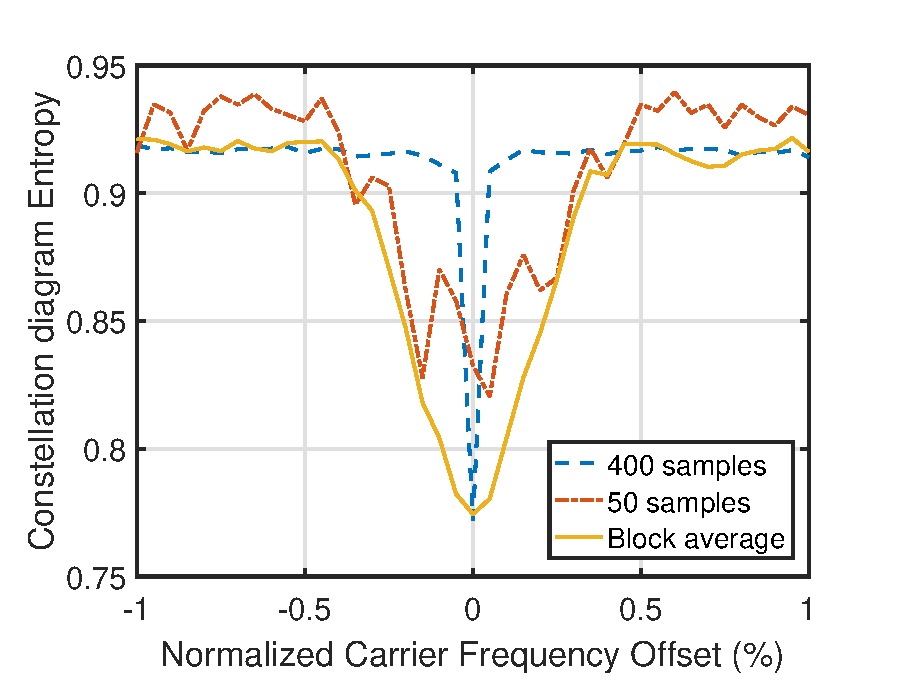
\includegraphics[width=3 in]{pic/freq.eps}
\caption{Constellation diagram entropy for carrier frequency recovery.}
\label{fig:freq_entp} 
\end{figure}   

% \subsubsection{Entropy Curve Expansion}
As can be observed in Fig. \ref{fig:freq_entp}, the entropy curve using 400 samples has only one global minimum when the CFO is equal to zero and no other local minima.
But its curve has a very narrow trough as predicted.
In comparison, the entropy estimated using 50 samples has a trough boundary at \(\pm 0.5\%\) of the symbol rate, which agrees with (\ref{eq:freq_limit}).
In fact, the trough range is expanded 8 times, but many fluctuations and local minima show up.
The entropy curve using the block average algorithm has the same expanded trough as the entropy estimated using 50 samples, but with smooth gradient without local minimum.

Given the expanded entropy trough, a more efficient two-step linear search can be readily applied.
First, a coarse search through the interested frequency range with a half trough width step size can give us an approximate CFO estimate.
A second search with a fine frequency step near the coarse estimation result provides an accurate CFO estimate.

Recall that the computation complexity grows quadratically with the number of samples, so breaking down the sample set into small blocks can significantly reduce the required computation.
In the previous case, if 400 samples is equally divided into 8 blocks, it is easy to find out that it only requires 1/8 of the total computation of Euclidean distance. 

% These EM based synchronization algorithms will be tested in controlled and realistic conditions in the nest section.

% In the above discussion, the CFO in each data batch is estimated and compensated,
% but the phase is not considered and there is phase discontinuity between batches.
% The initial phase of the data batch should be aligned with the last batch to ensure the phase continuity before the following carrier recovery.

% \subsubsection{Carrier Phase Continuity}
%     - only carrier frequency is recovered, phase different between blocks
%       - keep phase continuity between blocks

% \textbf{to be continued...}
% In high data-rate cases, the synchronization parameters
% (ε, θ, ω) vary slowly in comparison with the symbol interval.
% They can be assumed piecewise constant over a number of
% symbol periods. Synchronization of these quasi-constant parameters
% will be considered here, while tracking of the slowly
% varying parameters can be done in a post-processing unit [3].
%%%%%%%%%%%%%%%%%%%%%%%%%%%%%%%%%%%%%%%% The effect of various channel impairments will be analyzed on the system performance.  
%%%%%%%%%%
\section{Performance Evaluation}
\label{sec:perfo}
In this section, the performance of the synchronization algorithms presented in the previous section are assessed in controlled conditions.
In Section~\ref{sec:per_sim}, we will compare the timing and frequency estimation variance between the EM and ML algorithms.
The effect of various channel impairments
% , including noise, timing with CFO as well as multipath 
are analyzed on the system performance.
Finally, to examine the EM algorithm in realistic time varying channels, in Section~\ref{sec:per_sea}, it is applied to a set of data measured in a sea trial.

\subsection{Numerical Simulation}
\label{sec:per_sim}
% \subsection{Symbol Timing Performance}
First, we will examine performance of the symbol timing recovery algorithm (\ref{eq:ff_alg}) in presence of AWGN.
The O\&M algorithm is a batch mode, feedforward symbol timing estimator as described by (\ref{eq:om}).
% with the same structure as the proposed timing recovery algorithm~(\ref{eq:ff_alg}), 
Therefore, it is used here to represent the ML estimator in the performance comparison.

The performance comparison in presence of AWGN are shown in Fig. \ref{fig:timing_per}.
In this figure, both QPSK and 16-QAM modulation schemes are tested.
The RRC filter has a rolloff factor of 0.25. 
Complex AWGN is added to the received signal, such that the symbol energy to noise spectral density ratio (\(E_s/N_0\)) ranges from 5 to 40~dB with a step of 5~dB.
For each \(E_s/N_0\) setting, 500 Monte Carlo trials are tested.
In each trial, a block size of 100 samples are evaluated to estimate the TD.
After normalization by the symbol period, the timing error variances are plotted in the figure.
It is necessary to compare the results with the theoretical limit.
Following \cite{mengali1997synchronization}, the modified Cram\'er-Rao bound (MCRB) is also plotted as a reference.

\begin{figure}[ht]
\centering
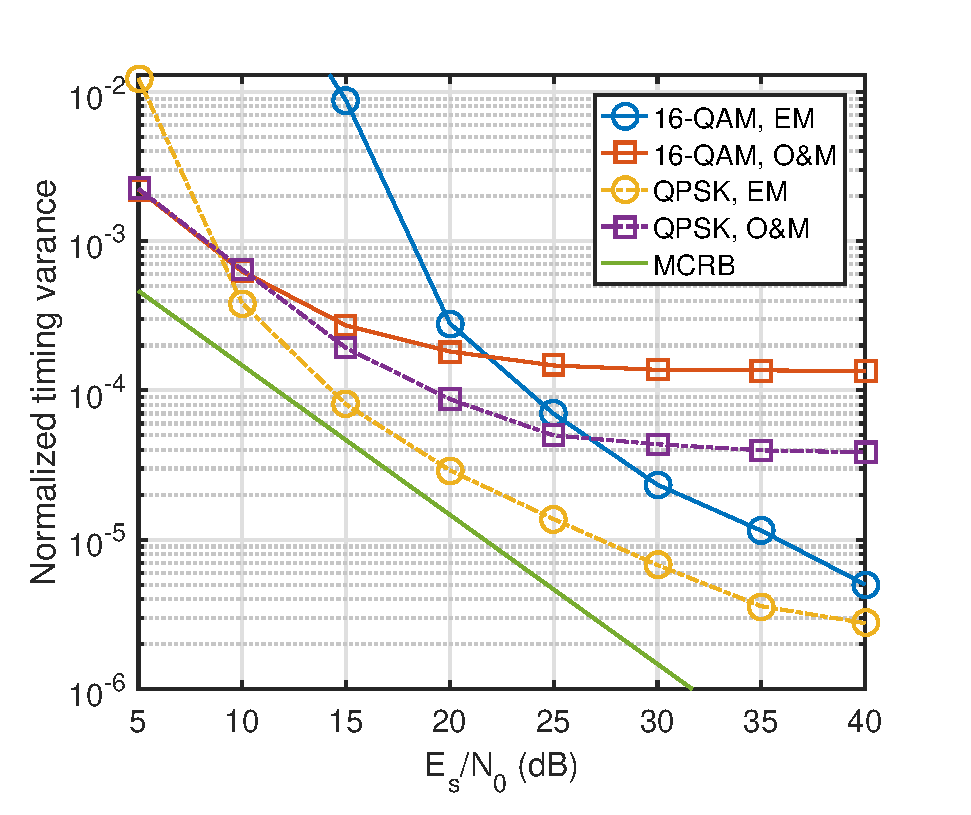
\includegraphics[width=3 in]{pic/per_timing.eps}
\caption{Performance of two symbol timing algorithms with 16-QAM and QPSK modulation schemes.}
\label{fig:timing_per} 
\end{figure}   

Several conclusions can be draw from this figure.
Generally speaking, when the  \(E_s/N_0\) is sufficiently high, the EM based symbol timing algorithm has lower variance than the O\&M algorithm for both QPSK and 16-QAM modulation schemes.
% This transition \(E_s/N_0\) is 8~dB for QPSK and 27~dB for 16-QAM
For both algorithms, the low modulation order tends to yield smaller timing variance.
% In the high \(E_s/N_0\) region, the performance of O\&M algorithm is limited by the self noise. 
When the \(E_s/N_0\) is greater than 25~dB, the O\&M reaches a lower boundary because of the strong self noise due to the small rolloff~\cite{mengali1997synchronization}. 
% * <x.liu@dal.ca> 2017-10-27T13:27:20.450Z:
% 
% the self noise is actually ISI, but they used this term in the citation to differentiate thermal noise
% 
% ^.
% When the \(E_s/N_0\) is greater than 25~dB, the strong self noise due to the small rolloff factor makes O\&M algorithm reaches its lower boundary, while 
In contrast, the EM algorithm keeps on improving with SNR, since the timing variance keeps getting smaller with the increased \(E_s/N_0\).
However, in low \(E_s/N_0\) region, the EM algorithm has inferior performance compared with ML algorithm.


Note that in the simulation, the rolloff factor is 0.25, which means the signal occupies relative small bandwidth but with significant ISI.
This scenario is in favour of EM based algorithm, since the eye diagram entropy estimation effectively measures the ISI.
However, if we have a larger rolloff factor, say 0.75, the O\&M algorithm will have a performance very close to the MCRB \cite{mengali1997synchronization}.
% * <x.liu@dal.ca> 2017-10-27T14:11:51.042Z:
% 
% at of the?
% 
% ^.
On the other hand, the enlarged signal bandwidth and reduced ISI make the EM based algorithm have inferior performance than the O\&M algorithm.

% \textit{Experiment 2: Performance of the symbol timing recovery in the presence of CFO.}
As explained in Section \ref{sec:timing}, the EM based symbol timing recovery is insensitive to the CFO, but it is interesting to understand how the performance changes in the presence of CFO. 
The settings are generally the same as the last simulation, but we will use BPSK and QPSK modulation schemes this time.
The introduced CFO is 1\% of the symbol rate, and the timing variances are plotted in Fig. \ref{fig:timing_frq_per}.

\begin{figure}[ht]
\centering
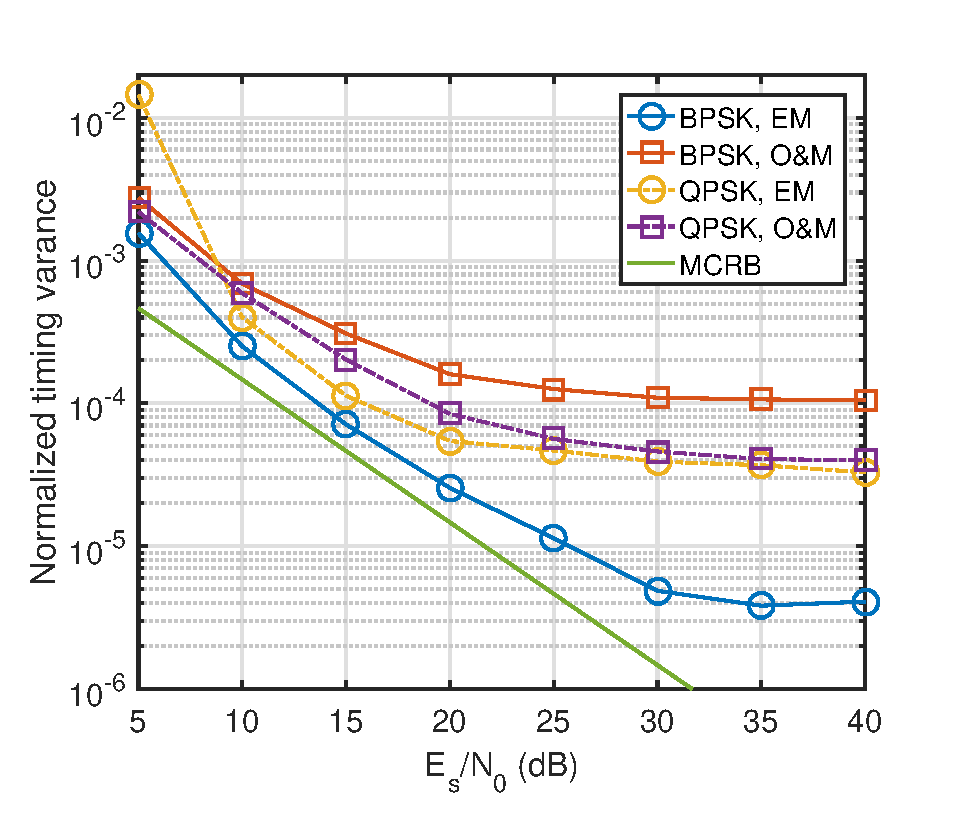
\includegraphics[width=3 in]{pic/per_timing_frq.eps}
\caption{Performance of two symbol timing algorithms in the presence of CFO.}
\label{fig:timing_frq_per} 
\end{figure}  

For BPSK modulation, EM based algorithm shows good performance that is close to the MCRB when the \(E_s/N_0\) is below 30 dB.
It has the highest performance improvement compared to O\&M.
However, for QPSK modulation, the performance improvement is marginal.
This is because the EM based algorithm in (\ref{eq:ff_alg}) assumes that the eye diagram entropy curve is symmetrical to the centre of the eye diagram, and this only stands with low modulation order and low noise level.
We will show another asymmetrical eye diagram entropy condition in the next simulation. 

% \textit{Experiment 3:EM based symbol timing recovery in multipath channel.}
One of the most important issue a single carrier coherent communication system facing is the multipath channel.
We will examine how the EM based symbol timing recovery performs in such condition.
Consider a set of BPSK modulated signal which is pulse shaped by the RRC filter with  a rolloff factor of 0.5.
For simplicity reason, the multipath channel considered here has has tow paths of arrival.
Its impulse response is given by
\begin{equation}
h(t)=\delta(t)-0.5(t-1.8T),
\end{equation}
and \(E_s/N_0\) at 25 dB.  
At the receiver, after the down converter and matched filter, the eye diagram and the corresponding entropy are shown in Fig. \ref{fig:per_timing_isi}. 
\begin{figure}[ht]
\centering
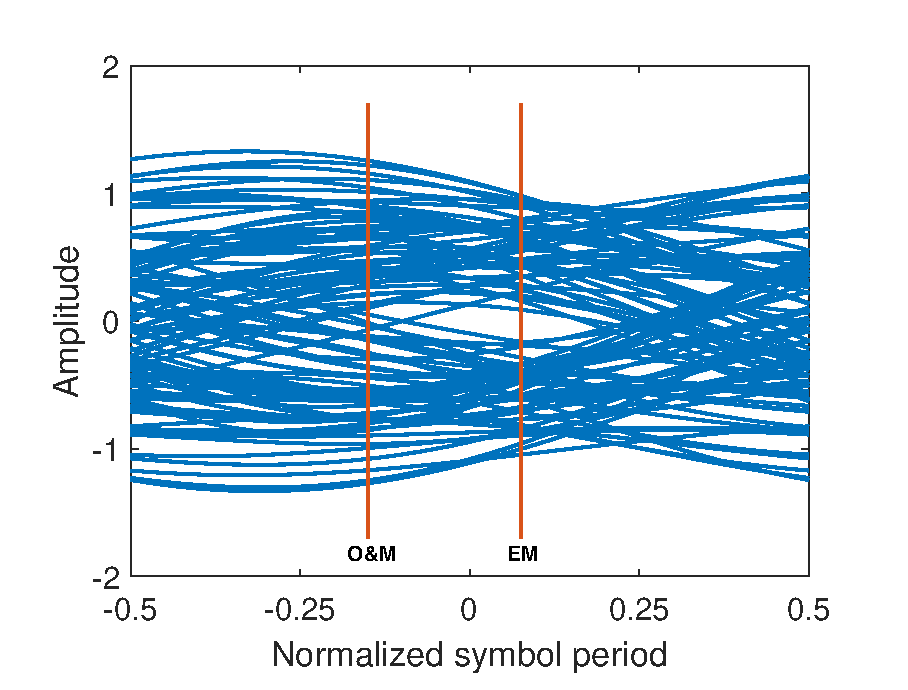
\includegraphics[width=3 in]{pic/per_timing_multi.eps}
\caption{An eye diagram after a multipath channel (upper) and the corresponding eye diagram entropy (lower).}
\label{fig:per_timing_isi} 
\end{figure} 

In the figure, there is no clear eye opening in the eye diagram, and the entropy curve is asymmetrical to the centre with one global and several local minimum. 
The timing instant with the global minimum is located at -0.1, where the eye diagram has three small eyes at their maximum opening.
The minimum entropy indicates that the least ISI is obtained in this timing instant.
With this timing instant choice, the equalizer can converge faster and produce stable results.
On the contrary, the timing instant found by ML based timing recovery algorithm is still around 0, 
where the output energy is maximized but with more random ISI.

Next, the performance of the carrier frequency recovery algorithms in the presence of AWGN will be evaluated.
In the carrier frequency recovery test, perfect symbol timing is assumed.
The signal is QPSK modulated with a CFO at 1\% of the symbol rate.
Two algorithms are compared to the EM based algorithm for CFO estimation:
the open loop and the ML algorithm.

% 红皮书 p105
The open loop algorithm proposed in \cite{Chuang1991} estimates the CFO  by averaging the differential phase error over the window.
For QPSK modulation scheme, the CFO is given by \cite{mengali1997synchronization}
\begin{equation}
f_\Delta = \frac{1}{8 \pi T} \arg \left\{ {\sum\limits_{i = 2}^{{N} - 1} {{{\big( {x_i x^*_{i-1}} \big)}^4}} } \right\}.
\label{eq:freq_openloop}
\end{equation}

The classic ML algorithm uses the same global search method as the EM algorithm.
The objective function is given by 
\begin{equation}
\Lambda (f_\Delta)=\left| \sum\limits_{i = 1}^N {{{ {{x^4_i}e^{-j8\pi f_\Delta i T}}}}} \right|^2. 
\label{eq:freq_ml}
\end{equation}
In (\ref{eq:freq_ml}), the CFO is estimated by searching for the trial CFO that yields the highest energy or alternatively by applying a computationally efficient FFT-based implementation \cite{Wang2004}.
Note that both (\ref{eq:freq_openloop}) and (\ref{eq:freq_ml}) are NDA algorithms and a power of 4 is applied to the signal to remove the modulation.
This is not necessary in the EM algorithm.
The CFO that is estimated using the three algorithms is normalized by the symbol rate,
and for each \(E_s/N_0\) condition, 500 trials are conducted to compute the variance.
The results are plotted in Fig. \ref{fig:per_freq}, where the MCRB is also included as the performance reference.

\begin{figure}[ht]
\centering
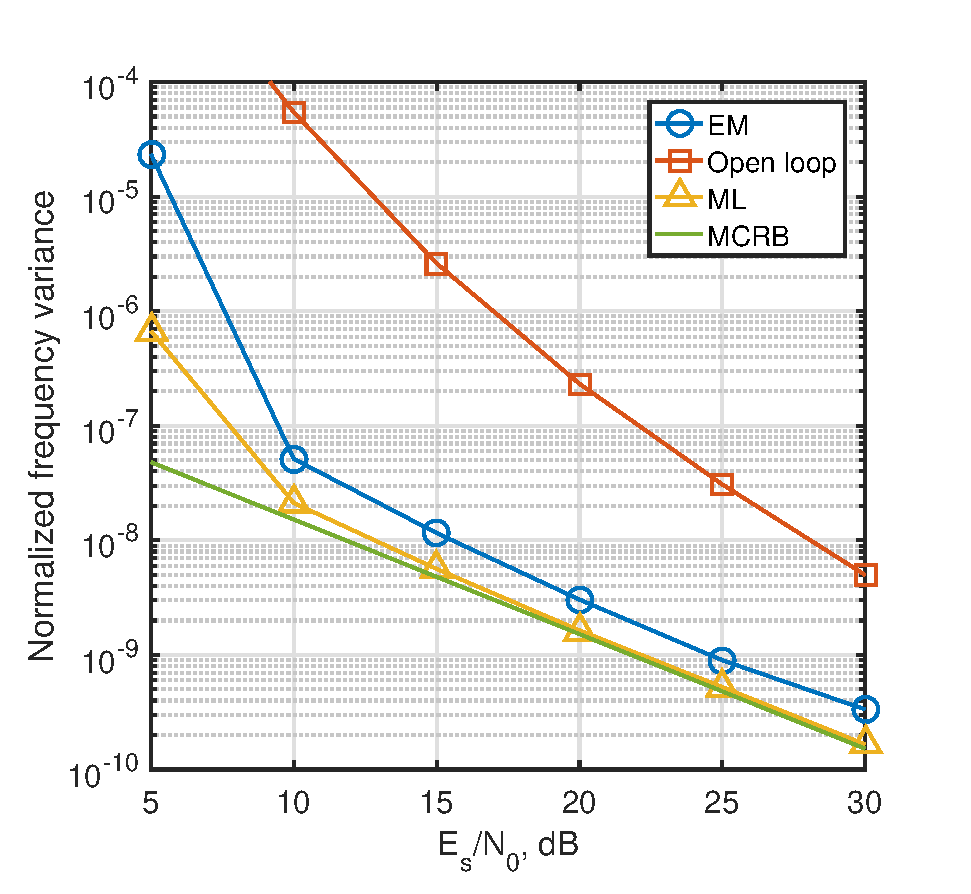
\includegraphics[width=3 in]{pic/per_freq.eps}
\caption{Performance of three carrier frequency recovery algorithms.}
\label{fig:per_freq} 
\end{figure} 


In the figure, the EM algorithm shows much smaller frequency variance than the open loop algorithm. 
This demonstrates its robust CFO estimation performance.
However, the performance of the ML algorithm is mostly the same as the MCRB, making it slightly better than the EM algorithm.
% When \(E_s/N_0\) is less than 10 dB, frequency variances of both the EM and ML algorithms grow 

There are several reasons why the the EM algorithm may have inferior performance in symbol timing and carrier recovery than the ML based algorithms.
First, the EM based algorithms (not the EM criterion itself) are derived under a few assumptions and approximations, which are not always true in practice.
The second reason is that the ML criterion is theoretically the optimum solution in AWGN channels, 
where the system can be characterized by the 2nd order statistics.
Its performance is supposed to reach the Cram\'er-Rao bound, therefore, the EM algorithms cannot achieve better performance.
The EM algorithms are more suitable for channels where high order statistics cannot be neglected.
% * <x.liu@dal.ca> 2017-10-27T13:58:44.114Z:
% 
% I want to differentiate the criterion from the algorithm.
% we should talk about this section
% 
% ^.

% test with sea trial measurement data
\subsection{Algorithm Validation with Sea Trial Data }
\label{sec:per_sea}
In this section, the EM based synchronization algorithms will be validated with realistic data measured in a sea trial. 
% \subsection{Sea Trial Environment and settings}
An underwater acoustic communication experiment took place in the Northwest Arm near Halifax, Canada on July 6th 2017. 
The experiment provided an opportunity to evaluate a variety of underwater communication algorithms.

In the test area, the depth is reported to be approximately 10-13 m, and the receiver's deployment location is around 220 m away from the transmitter.
The receiver drifts slowly because of the current.
% The sea state is favourable to the test. 
The acoustic propagation properties can also be observed using the channel impulse response in Fig. \ref{fig:chan_impu}, where there is a strong and stable direct path of arrival and a few multipath interference.
\begin{figure}[htbp]
\centering
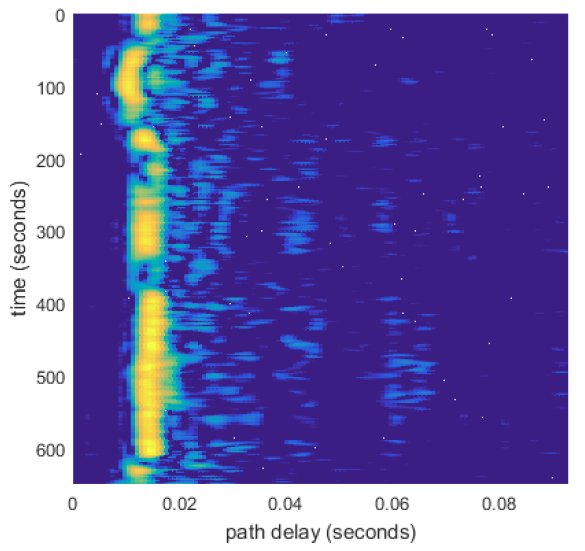
\includegraphics[width=2.5in]{pic/channel.png}
\caption{The timing varying channel impulse response.}
\label{fig:chan_impu} 
\end{figure}

A transmission frame is divided into pilot and data blocks. The pilot block is a wideband, linear frequency modulated chirp signal, which is used for frame synchronization.
The data block is divided into four sections, and each section has a symbol rate of 240, 80, 15 and 5 baud respectively. 
A pseudo-random noise (PN) sequence consisting of 512 symbols is used as the data content.
The modulation scheme is QPSK, and the transmitted waveform is pulse shaped using an RRC filter with a rolloff factor of 0.5. 
The carrier's centre frequency is 2.048~kHz. 

% \subsection{Data Processing Results}
% \label{sec:results}
At the receiver, all signals are sampled at 44.1~kHz. The frame is first coarsely synchronized with the pilot block so that the data block can be extracted.
Down conversion and a matched filter are applied to the data block to generate the complex baseband signal.

When the signal is demodulated without synchronization, the bit error rate (BER) is 51\%, which means no information is recovered.
To recover the data, EM based synchronization is applied.
For demonstration purposes, results from the 80 baud data are presented here.
In each iteration, 200 symbols are fed into the synchronizer to estimate the TD and CFO. 
The symbol timing and carrier frequency estimator outputs are shown in Fig. \ref{fig:per_exp}.

\begin{figure}[ht]
\centering
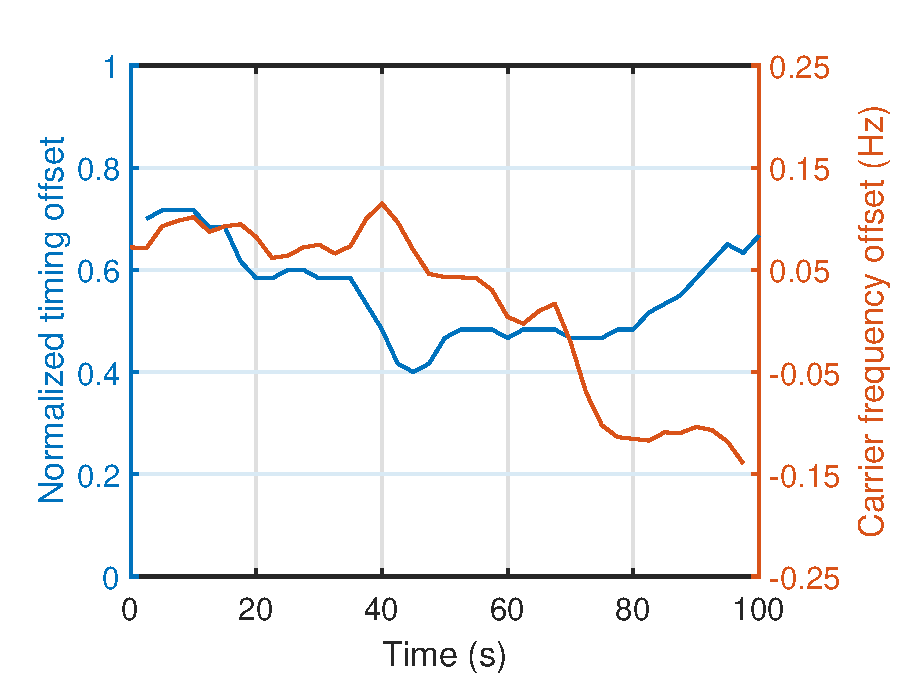
\includegraphics[width=3 in]{pic/per_exp.eps}
\caption{Symbol timing and carrier frequency estimation results from EM based algorithms.}
\label{fig:per_exp} 
\end{figure} 

% 先定时还是先频偏? 画出结果
% \begin{figure}[htbp]
% \centering
% \subfigure[Symbol timing offset as a function of time]{
% \label{fig:timing_result}
% \includegraphics[width=3.1in]{timoff.png}}
% % \hspace{0.2in} % 两图间距
% \subfigure[Carrier frequency offset as a function of time]{
% \label{fig:carrier_result}
% \includegraphics[width=3.1in]{freoff.png}}
% \caption{Synchronization results based on entropy minimization criterion.}
% \label{fig:sync_results} %% 总 label
% \end{figure}
There are totally 8192 QPSK symbols for a total duration of 102.4~s.
Both TD and CFO estimates are varying with time.
This is attributed to the Doppler effect due to the relative motion between the transmitter and the receiver.

% The synchronized data are depicted in Fig. \ref{fig:scatter}.
After demodulation, the BER is 0.41\%.
As a comparison, with conventional synchronization methods (pilot and PLL based), the BER is 0.49\%.
This result proves that the EM based synchronization algorithms are feasible and can reduce the communication system BER.
Note that the BER improvement is realized without equalization.  


%%%%%%%%%%%%%%%%%%%%%%%%%%%%%%%%%%%%%%%%%%%%%%%%%%
\section{Conclusions}
\label{sec:conc}
In this paper, a unified entropy minimization criterion is proposed for symbol timing and carrier frequency recovery in wireless coherent receivers.
It is an alternative to maximum likelihood criterion, which is the foundation of most of the standard synchronization algorithms. 
By exploring the high order statistics of the signal, entropy minimization is expected to possess superior performance. 

Synchronization is implemented by measuring the entropy of the eye diagram and the constellation.
% * <x.liu@dal.ca> 2017-10-27T14:07:10.265Z:
% 
% at of the?
% 
% ^.
The optimum timing delay is found by searching the timing instant with minimum eye diagram entropy, while the carrier frequency offset is estimated by searching through a range of frequencies and looking for the minimum constellation entropy.  

The histogram based entropy estimation method requires a large amount of computation.
In this paper, we proposed a customized fast entropy estimation algorithm.
It is a modified version of the quadratic R\'enyi entropy and the kernel density estimation method is employed to estimate the probabilities.

% Several practical issues are addressed when applying the entropy minimization criterion to signal synchronization.
Implementation constraints are also discussed in this paper. 
The proposed symbol timing algorithm can overcome local minimum, be insensitive to the carrier frequency offset, and extract timing delay without the need of high oversampling rate.
The carrier frequency recovery algorithm uses block averaging to expand the estimation range without compromising accuracy. 

The synchronization performance of the proposed algorithms is compared with standard approaches by running a set of numerical simulations.
It is shown that the entropy minimization criterion is more suitable in channels with  non-Gaussianity or non-linearity.
% * <x.liu@dal.ca> 2017-10-27T14:20:13.538Z:
% 
% help me with this sentence 
% 
% ^.
We also validated the algorithms with realistic data measured in a sea trial.
Good tracking and compensating results are received in a time varying underwater acoustic channel.
% \small
\bibliographystyle{IEEEbib}
\bibliography{Mendeley}


\end{document}